\section{Memory Efficient Convolutions}
\begin{figure}
	\centering
	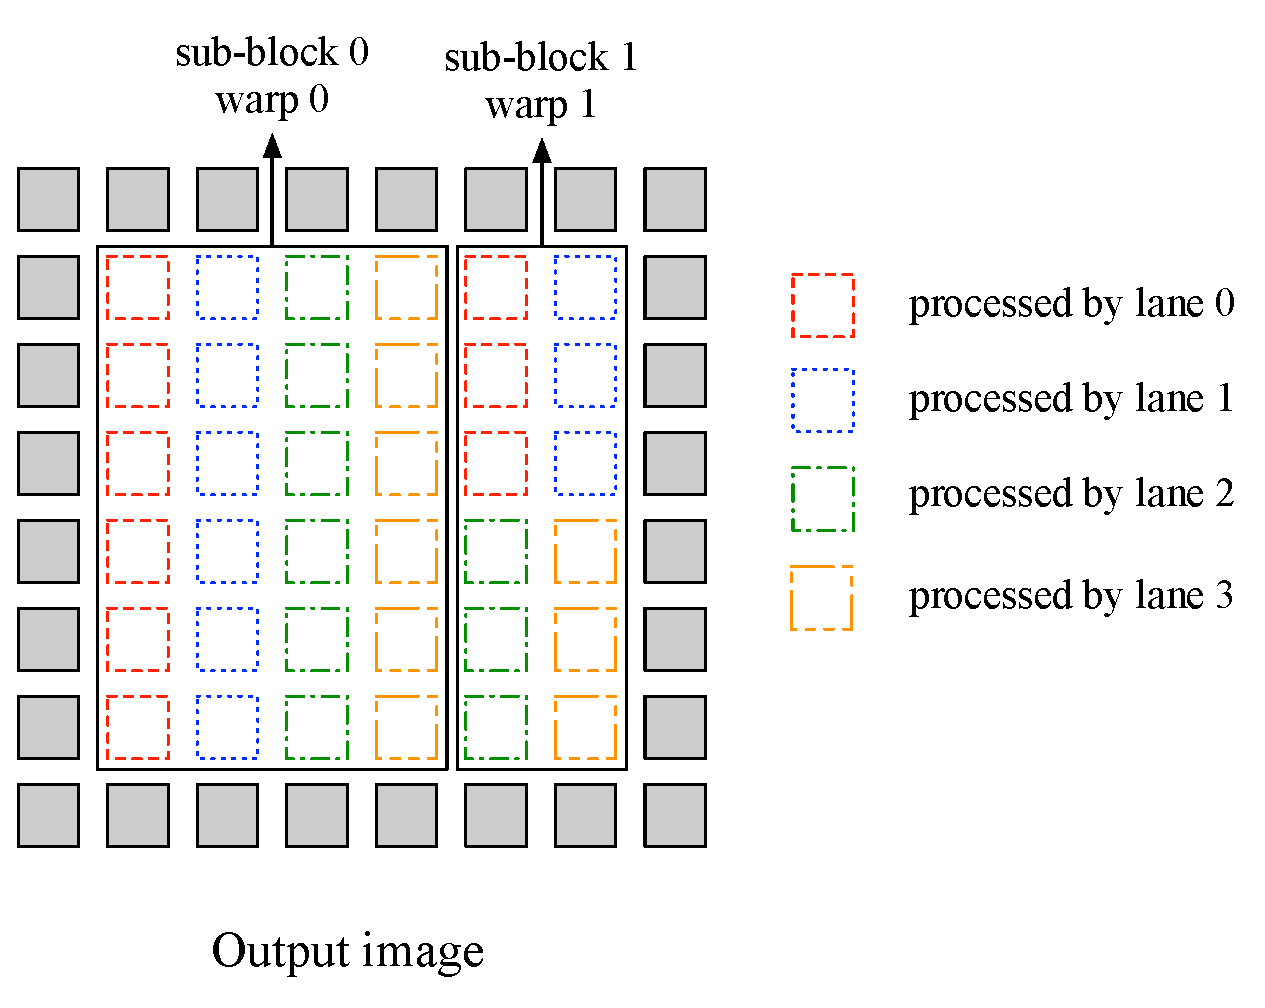
\includegraphics[width=0.9\columnwidth,height=5.5cm]{./figure/overalldesign.eps}
\caption{The output is produced by sliding a $3 \times 3$ filter over an $8 \times 8$ input with one pad. Edge elements and inner elements are processed by different thread blocks. We assume that the warp size is 4 and thus having $laneid=threadid\%4$.}
\label{fig:overalldesign}
\end{figure}


This section demonstrates the implementation of the two proposed reuse algorithms on convolution operations. {\color{red}As the 2D convolution is the basic operation of depth-wise and multi-channel 2D convolutions, we take the 2D convolution as an example to illustrate how to apply proposed reuse algorithms on convolution operations.}
%The main difference between the implementations in the 2D and 3D convolutions lies in the loading of filters. For the former, we focus on the scenario where a filter is used to slide over a large image. Therefore, we can load the entire filter into the shared memory, and only one thread block needs to load the filter once. For the latter, we focus on the scenario where many filters are used to slide over a batch of images, which are often the first layers of CNNs. All filters cannot fit into the shared memory; hence, we need to load the filters multiple times.

We first divide the output into sub-blocks, which contain exactly 32 (warp size) columns each, except for the last sub-block, which may contain less than 32 columns. {\color{red}We further divide a sub-block along height dimension if there are too many rows in it. Normally, each sub-block contains less than 56 rows.}
Each thread block processes one or more sub-blocks, and each warp processes one sub-block. The threads within the same warp process the adjacent columns of one sub-block.

\begin{algorithm}
	\KwIn{$I$, $F$, $subBlockHeight$}
	\KwOut{$O$}
	Load the filter into shared memory\;
	Divide columns of the filter into a combination of 3-column and 5-column sub-filters (only necessary for filter sizes larger than $5 \times 5$)\;
	$\_\_syncthreads()$\;
	\If{$blockIdx.x \textless gridDim.x-1$}{
		Init thread local register array $sum$ to zero\;
		Calculate the index of the first input element this thread needs, denoted as $inputIndex$\;
		\For{$i \gets 0$ \KwTo $subBlockHeight$}{
			\ForEach{sub-filter}{
				Load corresponding input elements from $inputIndex$ of global memory into $iTemp$\;
				Call $RetrieveThirdElement(iTemp)$ or $RetrieveSecondElement(iTemp)$\;
				Call $RowReuse(iTemp,i,$\textit{sub-filter}$,sum)$\;
			}
			Write completed element of $sum$ into $O$\;
		}		
		
	}
	\Else{
		Divide columns of the last sub-block into multiple partitions and try to evenly assign those partitions to threads of a warp. Each thread uses a direct method to calculate elements of $O$.\;
		The same method is adopted when processing the edge elements of $O$\;
	}
	\caption{2DConvolution}
	\label{algo:overalldesign}
\end{algorithm}

Figure \ref{fig:overalldesign} shows the mapping process of the threads onto output elements. Given that 2D convolutions normally produce an output image that has the same size as the input image, the latter should be padded. But we do not actually allocate memory on the GPU. We use different methods to calculate the edge and inner elements of the output. The edge and inner elements are represented by the shaded and dashed squares in Figure \ref{fig:overalldesign}, respectively.

%We also demonstrate how to deal with the inner elements and how to  calculate the edge elements using the same method for the inner elements. 
Each warp is assumed to contain four threads (Figure \ref{fig:overalldesign}). The inner elements are divided into two
sub-blocks. Sub-block 0 contains four columns, which represent the warp size, whereas sub-block 1 contains only two columns. To utilize the threads within a warp, we divide the last two columns evenly among the four threads. A generalized overall design is shown in Algorithm \ref{algo:overalldesign}.

We process the sub-blocks with exactly 32 columns and the last sub-block in Lines 4-15 and 16-19, respectively. Each thread calculates one column of output elements. First, each thread calculates the address of the first input element it needs (Lines 9). Second, each thread uses Algorithms \ref{algo:basic} and \ref{algo:basic2} to fulfill the row vector $iTemp$ (Line 10). Third, each thread passes the
vector $iTemp$ to Algorithm \ref{algo:rowreuse} to calculate multiple output elements and store results in register array $sum$ (Line 11).
At last, each thread writes the completed element of $sum$ into the result array $O$ (Line 13).


